\documentclass[tikz,border=10pt]{standalone}
\usepackage{tikz}
\usetikzlibrary{arrows.meta, positioning, fadings}

\begin{document}
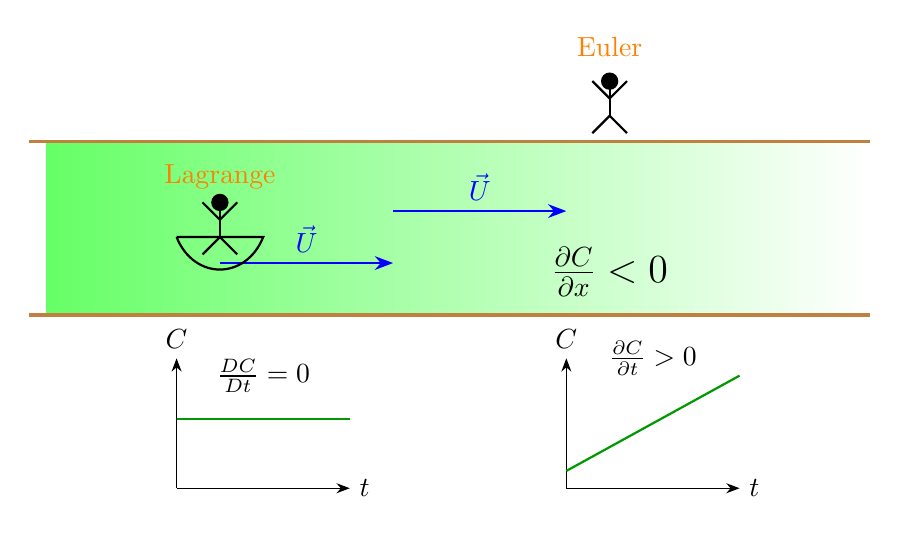
\begin{tikzpicture}[scale=1.1, >=Stealth]

% Custom fading for tracer gradient
\pgfdeclarehorizontalshading{tracer}{100bp}{
  color(0bp)=(green!70!white);
  color(100bp)=(green!10!white)
}
\pgfdeclarefading{tracerfade}{\pgfuseshading{tracer}}

% River background
%\fill[blue!5] (-0.5,1) rectangle (11.5,3);
%\fill[green!50, path fading=tracerfade, fading angle=0] (-0.5,1) rectangle (11.5,3);
\shade[left color=green, right color=white, opacity=0.6] (-0.5,1) rectangle (9,3);
\draw[very thick, brown] (-0.7,1) -- (9,1); % River bank
\draw[very thick, brown] (-0.7,3) -- (9,3); % River bank

% Flow arrow (left side)
\draw[->, thick, blue] (1.5,1.6) -- ++(2,0) node[midway, above] {$\vec{U}$};

% Flow arrow (right side)
\draw[->, thick, blue] (3.5,2.2) -- ++(2,0) node[midway, above] {$\vec{U}$};

% Gradient label
\node at (6,1.5) {\Large$\frac{\partial C}{\partial x} < 0$};

% Euler observer on bank
\begin{scope}[shift={(6,3.4)}]

  \fill (0,0.3) circle(0.1);
  \draw[thick] (0,0.3) -- (0,-0.1); % body
  \draw[thick] (0,-0.1) -- ++(-0.2,-0.2); % leg
  \draw[thick] (0,-0.1) -- ++(0.2,-0.2); % leg
  \draw[thick] (0,0.1) -- ++(-0.2,0.2); % arm
  \draw[thick] (0,0.1) -- ++(0.2,0.2); % arm
  \node[orange] at (0,0.7) {Euler};
\end{scope}
% Lagrange observer in boat (centered in river)
\begin{scope}[shift={(1.5,2)}]
  % Boat
  \begin{scope}[shift={(0,-0.5)}] % Shift down by 1 unit
  \draw[thick] (-0.5,0.4) .. controls (-0.3,-0.1) and (0.3,-0.1) .. (0.5,0.4)
             -- (-0.5,0.4); % upright hull
  \end{scope}
  % Person
  \fill (0,0.3) circle(0.1);
  \draw[thick] (0,0.3) -- (0,-0.1); % body
  \draw[thick] (0,-0.1) -- ++(-0.2,-0.2); % leg
  \draw[thick] (0,-0.1) -- ++(0.2,-0.2); % leg
  \draw[thick] (0,0.1) -- ++(-0.2,0.2); % arm
  \draw[thick] (0,0.1) -- ++(0.2,0.2); % arm
  \node[orange] at (0,0.6) {Lagrange};
\end{scope}

% Plots below

% Lagrange plot (left)
\begin{scope}[shift={(1, -1)}]
  \draw[->] (0,0) -- (2,0) node[right] {$t$};
  \draw[->] (0,0) -- (0,1.5) node[above] {$C$};
  \draw[thick, green!60!black] (0,0.8) -- (2,0.8);
  \node at (1,1.3) {$\frac{DC}{Dt} = 0$};
\end{scope}

% Euler plot (right)
\begin{scope}[shift={(5.5, -1)}]
  \draw[->] (0,0) -- (2,0) node[right] {$t$};
  \draw[->] (0,0) -- (0,1.5) node[above] {$C$};
  \draw[thick, green!60!black] (0,0.2) -- (2,1.3);
  \node at (1,1.5) {$\frac{\partial C}{\partial t} > 0$};
\end{scope}

\end{tikzpicture}
\end{document}
